\documentclass[9pt,handout]{beamer}

\input{./StyleFile.tex}

% \setbeameroption{show notes}
% \setbeameroption{show notes on second screen=right}

\title[\textbf{Resilient Machine Learning Approaches for Fast Risk Evaluation and Management in Financial Portfolios and Variable Annuities}]{Efficient Machine Learning Approaches for Fast Risk Evaluation of VAs}

\author[\textbf{Xintong Li, xintong.li1@uwaterloo.ca}]
{\Large\bfseries
Xintong Li\\\medskip
xintong.li1@uwaterloo.ca
} % Your name

\institute[\textbf{University of Waterloo, Actuarial Science}] % Your institution as it will appear on the bottom of every slide, may be shorthand to save space
{\large\bfseries
Dept. Statistics and Actuarial Science\\\smallskip
University of Waterloo % Your institution for the title page
}


\jointwork{Supervised by Prof. Tony Wirjanto and Prof. Mingbin Feng}
\conference{Thesis Defense, University of Waterloo}


%\usepackage[backend=bibtex,citestyle=authoryear-icomp,natbib,maxcitenames=1]{biblatex}
%\addbibresource{NestedSim.bib}

% use this so appendices' page numbers do not count
\usepackage{appendixnumberbeamer}
\usepackage{booktabs}
\usepackage[round]{natbib}
\usepackage{mathtools}
% \usepackage{subfigure}


\usepackage{amsmath}
\usepackage{amsfonts}
\usepackage{amssymb}
\usepackage{bbm}
\usepackage{xcolor}
\usepackage{algorithm}
\usepackage{algorithmic}
\usepackage{subcaption}
\usepackage{graphicx}
\usepackage{bm}

\usepackage{tikz}
\usetikzlibrary{shapes,arrows,positioning, calc, fit, decorations.pathreplacing}




\definecolor{color10_2}{HTML}{1F77B4}
\definecolor{color10_3}{HTML}{FF7F0E}
\definecolor{color10_4}{HTML}{2CA02C}
\definecolor{color10_5}{HTML}{D62728}
\definecolor{color10_6}{HTML}{9467BD}
\definecolor{color10_7}{HTML}{8C564B}
\definecolor{color10_8}{HTML}{E377C2}
\definecolor{color10_9}{HTML}{7F7F7F}
\definecolor{color10_10}{HTML}{BCBD22}
\definecolor{color10_11}{HTML}{17BECF}


\newtheorem{assumption}{Assumption}
\newtheorem{proposition}{Proposition}

\DeclarePairedDelimiter\ceil{\lceil}{\rceil}
\DeclarePairedDelimiter\floor{\lfloor}{\rfloor}

\begin{document}

% Title page, navigation surpressed, no page number
{
\beamertemplatenavigationsymbolsempty
\begin{frame}[plain]
\titlepage
\end{frame}
}

{
\beamertemplatenavigationsymbolsempty
\defbeamertemplate*{headline}{miniframes theme no subsection no content}
{ \begin{beamercolorbox}{section in head/foot}
    \vskip\headheight
  \end{beamercolorbox}}
\begin{frame}{Outline}
\tableofcontents
\end{frame}
}
\addtocounter{framenumber}{-2}


\section{Introduction}

\begin{frame}{Nested Simulation Procedures}

Nested simulation procedures are necessary for \textbf{complex} financial derivatives and insurance products.

$$\rho(L) = \rho(L(X)), \;\;\; L(X) = \mathbb{E}\left[ Y|X=x \right]\vert_{x=X}  $$

Involves two levels of Monte Carlo simulations:
\begin{itemize}
    \item Outer level: generates underlying risk factors (outer scenarios), $X_i \sim F_X$
    \item Inner level: generates scenario-wise samples of portfolio losses (inner replications), $Y_{ij} \sim F_{Y|X_i}$
\end{itemize}

\textbf{Computationally expensive due to its nested structure.}

\end{frame}

\begin{frame}{Common Risk Measures}

\begin{itemize}
    \item Smooth $h$, e.g., quadratic tracking error

    $$ \rho(L) = \mathbb{E} \left[ (L - b)^2 \right] $$
    
    \item hockey-stick $h$: mean excess loss
    
    $$ \rho(L) = \mathbb{E} \left[ L \cdot \mathbbm{1}_{\{L \geq u\}} \right] $$
    
    \item indicator $h$: probability of large loss
    
    $$ \rho(L) = \mathbb{E} \left[ \mathbbm{1}_{\{L \geq u\}} \right] $$
    
    \item Value at Risk (VaR)
    
    $$ \rho_\alpha(L) = Q_\alpha(L) = \inf \{ u: \mathbb{P}(L \leq u) \geq \alpha \} $$
    
    \item Conditional Value at Risk (CVaR) \footnotemark
    
    $$ \rho_\alpha(L) = \mathbb{E} \left[ L \vert L \geq Q_\alpha(L) \right] $$

    \end{itemize}

    \footnotetext{Note: If $Q_\alpha(L)$ falls in a probability mass, $\rho(L) = \frac{(\beta - \alpha)Q_\alpha(L) + (1- \beta) \mathbb{E} \left[ L \vert L \geq Q_\alpha(L) \right]}{1-\alpha}$.}

\end{frame}

\section{Nested Simulation Procedures in Financial Engineering: A Selected Review}

\begin{frame}{Standard Nested Simulation}

$$\hat{L}_{N, i} = \frac{1}{N} \sum_{j=1}^N Y_{ij}; ~~~ Y_{ij} \sim F_{Y|X_i} $$

\begin{itemize}
    \item Uses inner sample mean to estimate $L(X_i)$.
    \item Proposed by \citet{gordy2010nested}; finds optimal growth order of $M$ and $N$.
    \item \citet{zhang2021bootstrap} estimate the optimal $M$ and $N$ using a bootstrap method.
    \item Computationally expensive and potentially \textbf{wasteful} use of budget.
\end{itemize}

\end{frame}

\begin{frame}{Other Nested Simulation Procedures}

Subsequent works focus on improving the efficiency of nested simulation:
\begin{itemize}
    \item Regression-based~\citep{broadie2015risk}
    \item Kernel smoothing~\citep{hong2017kernel}
    \item Likelihood ratio~\citep{feng2020optimal}
    \item Kernel ridge regression~\citep{zhang2022sample}
\end{itemize}

\vspace{10pt}

\textbf{Key ideas:} 
\begin{itemize}
    \item Pool inner replications from different outer scenarios 
    \item Use metamodeling techniques to approximate the inner simulation model
\end{itemize}

\end{frame}

\begin{frame}{Metamodeling Approach}

In this thesis, we focus on procedures that use \textbf{supervised learning metamodels} to approximate the inner simulation model.   

\begin{itemize}
    \item Treat the inner simulation as a black-box function
    \item Approximate $L(\cdot)$ with $\hat{L}^{\text{SL}}_{M, N}(\cdot)$
    \item Train with a set of feature-label pairs generated from the standard procedure:
    $$\{(X_i, \hat{L}_{N, i}) \vert i=1, \ldots, M, j=1, \ldots, N\}$$
    \item Use trained metamodel to make predictions for all $X \in \mathcal{X}$
\end{itemize}

There are \textbf{computational costs} associated with pooling inner replications.

\end{frame}


\begin{frame}{Problem Statement}

Minimize mean squared error (MSE) of the estimator subject to total simulation budget:

\begin{align*}
\min_{M, N} ~~~ \mathbb{E} \left[ \left( \hat{\rho}_{M, N} - \rho \right)^2 \right] \\
\text{ subject to } M \cdot N = \Gamma
\end{align*}

Interested in convergence order as $\Gamma \to \infty$

\end{frame}

\subsection{Theoretical Results}

\begin{frame}{Asymptotic Convergence Rates of Different Procedures}

    \begin{table}
		\centering
		\begin{tabular}{l|c|c|c}
			\toprule
			\textbf{Procedures} & \textbf{Smooth $h$} & \textbf{Hockey-Stick $h$} & \textbf{Indicator $h$}  \\
			\midrule
			Standard Procedure	& \textcolor{red}{$\mathcal{O}(\Gamma^{-2/3})$} & \textcolor{red}{$\mathcal{O}(\Gamma^{-2/3})$} & $\mathcal{O}(\Gamma^{-2/3})$ \\
			\midrule
			Regression  & $\mathcal{O}(\Gamma^{-1})$ & $\mathcal{O}(\Gamma^{-1+\delta})$ & No Result \\
			\midrule
			Kernel Smoothing 	& \multicolumn{3}{c}{$\mathcal{O}(\Gamma^{-\min(1, 4/(d+2))})$}  \\
			\midrule
			Kernel Ridge Regression  		& \multicolumn{3}{c}{$\mathcal{O}(\Gamma^{-1})$} \\
			\midrule
			Likelihood Ratio  			& \multicolumn{3}{c}{$\mathcal{O}(\Gamma^{-1})$} \\
			\bottomrule
		\end{tabular}
	\end{table}
    \vspace{10pt}
    \begin{itemize}
        \item We show the asymptotic convergence rates of the standard procedure for smooth and hockey-stick $h$.
        \item Only kernel smoothing depends on the asset dimension $d$.
    \end{itemize}
    
\end{frame}

\begin{frame}{Key Theoretical Results}

\textbf{Observations:}
\begin{itemize}
\item Most literature focuses on the MSE of $\hat{\rho}$.
\item \citet{wang2022smooth} analyze convergence of absolute error in probabilistic order.
\end{itemize}

\vspace{10pt}

\textbf{Contribution:} bridging the gap between MSE and absolute error convergence.
\begin{itemize}
    \item Convergence in MSE:
    $$ \mathbb{E} \left[ \left( \hat{\rho}_{\Gamma} - \rho \right)^2 \right] = \mathcal{O} \left( \Gamma^{-\xi} \right) $$
    \item Convergence in Probabilistic Order:
    $$ |\hat{\rho}_{\Gamma} - \rho| = \mathcal{O}_{\mathbb{P}}(\Gamma^{-\xi}) $$
\end{itemize}

\end{frame}

\begin{frame}{Key Theoretical Results}

\begin{block}{Theorem}
    If $\hat{\rho}_{\Gamma}$ converges in MSE to $\rho$ in order $\xi$, then $\hat{\rho}_{\Gamma}$ converges in probabilistic order to $\rho$ in order $\frac{\xi}{2}$.
\end{block}

\begin{itemize}
    \item First result to draw connection between MSE and probabilistic order convergence.
    \item Applicable to any nested simulation procedure.
    \item Convergence in MSE implies convergence in probabilistic order.
\end{itemize}

\end{frame}

\subsection{Finite-Sample Analysis}

\begin{frame}{Experiment Design}

We compare 5 nested simulation procedures 
\begin{itemize}
    \item Standard nested simulation
    \item Regression-based
    \item Kernel smoothing
    \item Likelihood ratio
    \item Kernel ridge regression
\end{itemize}

And their empirical convergence stable across different:
\begin{itemize}
    \item Risk measures
    \item Option types
    \item Asset dimensions
    \item Asset models (GBM vs. Heston)
    \item Regression bases (only for the regression-based procedure)
\end{itemize}

\end{frame}

\begin{frame}{Finite-Sample Performance}

\begin{figure}
    \includegraphics[width=\textwidth]{../project1/figures/figure1.png}
    \caption{Empirical convergence rates of different procedures for the base case}
\end{figure}

\end{frame}

\begin{frame}{Sensitivity to Asset Dimension}

\begin{figure}
    \includegraphics[width=\textwidth]{../project1/figures/figure2a.png}
\end{figure}

\begin{itemize}
    \item Standard, KRR, and likelihood ratio procedures are dimension-independent
    \item Kernel smoothing and regression show sensitivity to dimension, but in different ways
\end{itemize}

\end{frame}

\begin{frame}{Sensitivity to Asset Dimension}

    \begin{figure}
        \includegraphics[width=\textwidth]{../project1/figures/figure2b.png}
    \end{figure}
    
    \begin{itemize}
        \item Standard, KRR, and likelihood ratio procedures are dimension-independent
        \item Kernel smoothing and regression show sensitivity to dimension, but in different ways
    \end{itemize}
    
\end{frame}

\begin{frame}{Fast Convergence of Regression-based Procedure}

\begin{figure}
    \includegraphics[width=\textwidth]{../project1/figures/figure3.png}
\end{figure}

\begin{itemize}
    \item Higher initial convergence rate
    \item Stabilizes to match asymptotic rate at higher budgets
    \item Consistent across different asset dimensions
\end{itemize}

\end{frame}

\begin{frame}{Sensitivity to Option Type}

\begin{figure}
    \includegraphics[width=\textwidth]{../project1/figures/figure6a.png}
\end{figure}

\begin{itemize}
    \item Similar convergence patterns across different option types
    \item Regression and kernel smoothing show higher empirical rates for barrier options
\end{itemize}

\end{frame}

\begin{frame}{Sensitivity to Risk Measure}

\begin{figure}
    \includegraphics[width=\textwidth]{../project1/figures/figure8a.png}
\end{figure}

\begin{itemize}
    \item Convergence behavior consistent across different risk measures
    \item Regression-based method shows highest empirical convergence rates
\end{itemize}

\end{frame}

\begin{frame}{Sensitivity to VaR/CVaR Level}

\begin{figure}
    \includegraphics[width=\textwidth]{../project1/figures/figure9a.png}
\end{figure}

\begin{itemize}
    \item Regression-based method not sensitive to VaR/CVaR level
    \item Consistent performance across different levels
\end{itemize}

\end{frame}

\begin{frame}{Sensitivity to Asset Model}

\begin{figure}
    \includegraphics[width=\textwidth]{../project1/figures/figure10a.png}
\end{figure}

\begin{itemize}
    \item Regression-based method insensitive to asset model (GBM vs. Heston)
    \item Consistent performance across different asset models
\end{itemize}

\end{frame}

\begin{frame}{Computational Complexity}

    There are \textbf{computational costs} associated with pooling inner replications.

    \begin{itemize}
        \item Standard procedure: cost of estimating the optimal $M$ and $N$
        \item Regression: most efficient among metamodel-based procedures
        \item Kernel smoothing: costly distance calculations and cross-validation
        \item Likelihood ratio: No training, but costly weight calculations
        \item KRR: even more expensive than kernel smoothing
    \end{itemize}

\end{frame}

\begin{frame}{Total Computation Time}

    \begin{figure}
        \includegraphics[width=\textwidth]{../project1/figures/figure11b.png}
        \caption{Total computation time for different procedures}
    \end{figure}

\end{frame}

\begin{frame}{Cost of Hyperparameter Tuning}

    \begin{figure}
        \includegraphics[width=\textwidth]{../project1/figures/figure12a.png}
        \caption{Cost of hyperparameter tuning for different procedures}
    \end{figure}

\end{frame}

\begin{frame}{Cost of Model Fitting and Validation}

    \begin{figure}
        \includegraphics[width=\textwidth]{../project1/figures/figure12b.png}
        \caption{Cost of model fitting and validation for different procedures}
    \end{figure}

\end{frame}

\begin{frame}{Conclusion}
    Regression-based nested simulation procedure:
    \begin{itemize}
        \item Most robust and stable for limited budgets
        \item Efficient to implement
        \item Fast empirical convergence for option portfolios
    \end{itemize}

    \vspace{10pt}

    For high-dimensional or complex payoffs:
    \begin{itemize}
        \item Difficult to find a good regression basis
        \item Neural network-based procedures may be more suitable
    \end{itemize}

    \vspace{10pt}

    Next project: examining performance of metamodel-based simulation procedures for variable annuities


\end{frame}

\section{Using Deep Neural Network Metamodels for High-Dimensional Nested Simulation}

\begin{frame}{From Options to Variable Annuities}

    Variable annuities (VAs) poses a challenge for nested simulation due to its \textbf{high-dimensional} and \textbf{complex payoff structure}.

    \vspace{10pt}

    \begin{figure}[H]
            \includegraphics[width=0.33\textwidth]{./tikz/illustration_spns.pdf}
            \includegraphics[width=0.62\textwidth]{./tikz/illustration_mpns.pdf}
	\end{figure}

    \vspace{10pt}

    \begin{itemize}
        \item Need to reconstruct a metamodeling-based nested simulation procedure
    \end{itemize}

\end{frame}

\begin{frame}{Nested Simulation for Risk Management of VAs}

    \begin{figure}[c]
        \includegraphics[width=\textwidth]{../project2/figures/sns.pdf}
        \caption{Illustration of nested simulation that estimates the P\&L for one outer scenario}
    \end{figure}


\end{frame}

\begin{frame}{Standard Nested Simulation for VAs}

Standard nested simulation for VAs is similar to the one for options.

\begin{itemize}
    \item Generate $M$ outer scenarios
    \item For each outer scenario,
    \begin{itemize}
        \item Perform $N$ inner simulations
        \item Estimate hedging loss $L_i$ with $\hat{L}_i$
    \end{itemize}
    \item Use estimated losses to calculate tail risk measures (e.g., $95\%$-CVaR)
\end{itemize}

\vspace{10pt}

\textbf{Observations:}
\begin{itemize}
    \item computational budget is limited;
    \item high-dimensional input space;
    \item only a \textbf{small} portion of scenarios are relevant when estimating \textbf{tail} risk measures.
\end{itemize}

\end{frame}

\begin{frame}{Metamodel-based Nested Simulation}

    We use deep neural networks (DNNs) as metamodels 
    \begin{itemize}
        \item Use LSTMs for sequential data
        \item \textbf{Challenge}: lack of transparency and interpretability
    \end{itemize}

    \vspace{20pt}

    \textbf{Research Contributions:}
    \vspace{6pt}
    \begin{enumerate}
        \item Propose two generic DNN-based nested simulation procedures
        \begin{itemize}
            \item   Accurate tail scenario identification
            \item   Significant computational savings by \textbf{budget concentration}
        \end{itemize}
        \vspace{6pt}
        \item Study noise tolerance of DNNs using simulated data
        \begin{itemize}
            \item \textbf{Control noise levels} by adjusting simulation parameters
            \item Provide direct evidence on transparency and interpretability
        \end{itemize}
    \end{enumerate}

\end{frame}

\begin{frame}{Two-Stage Metamodel-based Nested Simulation}

\begin{algorithm}[H]
    \caption{Two-Stage Metamodel-based Nested Simulation for VAs}

\begin{algorithmic}[1]
    \STATE{\textbf{Generate training data for metamodels:}}
    \begin{itemize}
        \item Use a fraction of the simulation budget to run the standard nested simulation procedure with $M$ outer scenarios and $N'$ inner replications.
        \item Construct feature-label pairs $\{(X_i, Y_{ij}) : i=1, \ldots, M, j=1, \ldots, N'\}$
    \end{itemize}
    \STATE{\textbf{Train metamodels:}}
    \begin{itemize}
        \item Use the feature-label pairs to train a metamodel.
        \item Use the trained metamodel to make predictions for $\{X_i: i=1, \ldots, M\}$.
        \item Sort the predicted losses to identify a predicted tail scenario set that contains the $m$ largest predicted losses.
    \end{itemize}
    \STATE{\textbf{Concentrate simulation on predicted tail scenarios:}}
    \begin{itemize}
        \item Run the standard procedure on the predicted tail scenarios.
        \item Estimate the $\alpha$-CVaR of $L$ using the estimated losses on the predicted tail scenarios.
    \end{itemize}
\end{algorithmic}
\end{algorithm}

\end{frame}


\begin{frame}{Benefits of a Two-Stage Procedure}


Simulation budget can be saved when:
\begin{itemize}
    \item the metamodel is accurate (a small $m$ includes most tail scenarios)
    \item the metamodel can tolerate noise in training labels (a small $N'$)
\end{itemize}

\vspace{10pt}

\textbf{Key findings:}
\begin{itemize}
    \item Substantial computational savings ($70\% - 85\%$ reduction)
    \item Maintains accuracy comparable to standard procedure
    \item DNN metamodels can distinguish between tail and non-tail scenarios effectively
    \item Addresses regulatory concerns by using actual simulations for final estimates
\end{itemize}

\vspace{10pt}
\textbf{Another finding:} 
some DNN metamodels make \textbf{accurate loss predictions} for given scenarios.

\end{frame}

\begin{frame}{Single-Stage Metamodel-based Nested Simulation}

\begin{algorithm}[H]
\caption{Single-Stage Metamodel-based Nested Simulation for VAs}
\begin{algorithmic}[1]
    \STATE{\textbf{Generate training data for metamodels:}}
    \begin{itemize}
        \item Use the entire simulation budget to run the standard nested simulation procedure with $M$ outer scenarios and $N$ inner replications.
        \item Construct feature-label pairs $\{(X_i, Y_{ij}) : i=1, \ldots, M, j=1, \ldots, N\}$
    \end{itemize}
    \STATE{\textbf{Train metamodels:}}
    \begin{itemize}
        \item Use the feature-label pairs to train a metamodel.
        \item Use the trained metamodel to make predictions for $\{X_i: i=1, \ldots, M\}$.
    \end{itemize}
    \STATE{\textbf{Use metamodel predictions to estimate tail risk measures directly.}}
\end{algorithmic}
\end{algorithm}

\textbf{Key advantages:}
\begin{itemize}
    \item more efficient than a two-stage procedure;
    \item avoids specifying $m$.
\end{itemize}

\end{frame}

\begin{frame}{Experiment Setting}

    We estimate the $95\%$-CVaR of the hedging loss for a GMWB contract with 20-year maturity.

    \vspace{10pt}

    \textbf{Specifications:}
    \begin{itemize}
        \item The underlying asset follows a regime-switching geometric Brownian motion;
        \item The contract is delta-hedged monthly (240 periods);
        \item The true $95\%$-CVaR is estimated using 100,000 outer scenarios and 100,000 inner replications.
        \item The metamodel is trained using 90,000 outer scenarios and 100 inner replications.
        \item Benchmark: standard nested simulation procedure with 100,000 outer scenarios and 1,000 inner replications.
    \end{itemize}

\end{frame}

\begin{frame}{Experiment Design}

    \textbf{Research Questions:}
    \begin{itemize}
        \item What do DNNs learn from noisy data?
        \item How well do DNNs learn from noisy data?
    \end{itemize}

    \begin{figure}[H]
        \includegraphics[width=\textwidth]{../project2/figures/datasets.png}
    \end{figure}

    \begin{itemize}
        \item Our 90,000 training data is noisy, and the test data is also \textbf{noisy}.
        \item Our evaluation is based on the true (\textbf{noiseless}) feature-label relationship\footnotemark.
    \end{itemize}

    \footnotetext{Made possible by novel simulation design.}

\end{frame}

\begin{frame}{Experiment Setting}

    We consider the following metamodel architectures:

    \begin{table}[ht!]
        \centering
        \begin{tabular}{lcc}
            \toprule
            \textbf{Metamodel} & \textbf{Abbreviation} & \textbf{Capacity} \\
            \midrule
            Multiple Linear Regression      & MLR       & 241 \\
            Quadratic Polynomial Regression & QPR       & 481 \\
            Feedforward Neural Network      & FNN       & 35,009 \\
            Recurrent Neural Network        & RNN       & 32,021 \\
            Long Short-Term Memory          & LSTM      & 35,729 \\
            \bottomrule
        \end{tabular}
        \caption{Metamodel architectures for GMWB inner simulation model}
        \label{tab:arch}
    \end{table}

    Capacity is defined as the number of parameters in the metamodel.
    \begin{itemize}
        \item   Higher capacity metamodels are more flexible and expressive.
        \item   Lower capacity metamodels are less likely to overfit.
    \end{itemize}
    
\end{frame}

\begin{frame}{Traditional Regression Metamodels}

    \begin{figure}[H]
        \includegraphics[width=0.48\textwidth]{../project2/figures/qqPlots/mlrLN.png}
        \includegraphics[width=0.48\textwidth]{../project2/figures/qqPlots/qprLN.png}
        \caption{QQ plots between true and predicted loss labels for MLR and QPR metamodels}
    \end{figure}

    \begin{itemize}
        \item   MLR and QPR metamodels make \textbf{inaccurate} loss predictions.
        \item   Feature engineering is hardly feasible for our 240-dimensional $X$.
    \end{itemize}

\end{frame}

\begin{frame}{Deep Neural Network Metamodels}

    \begin{figure}[H]
        \includegraphics[width=0.48\textwidth]{../project2/figures/qqPlots/fnnLN.png}
        \includegraphics[width=0.48\textwidth]{../project2/figures/qqPlots/lstmLoCapLN.png}
        \caption{QQ plots between true and predicted loss labelsfor FNN and LSTM metamodels}
    \end{figure}

    \begin{itemize}
        \item   DNN metamodels are more flexible.
        \item   Time series features prefer a LSTM metamodel over FNN.
        \item   Network architecture serves as prior knowledge that regularizes DNNs.
    \end{itemize}

\end{frame}

\begin{frame}{Metamodel Performance on Different Datasets}

    \begin{table}[ht!]
        \centering
        \small
        \begin{tabular}{lccc}
        \toprule
        \textbf{Metamodel} & \textbf{Training error} & \textbf{Test error} & \textbf{True error}\\
        \midrule
        MLR & $0.706 (\pm 8.34\times 10^{-4})$ & $0.713 (\pm 2.67 \times 10^{-2})$ & $0.706 (\pm 3.44 \times 10^{-4})$ \\
        QPR & $0.543 (\pm 8.27\times 10^{-4})$ & $0.554 (\pm 2.32 \times 10^{-2})$ & $0.544 (\pm 4.12\times 10^{-4})$ \\
        FNN & $0.129 (\pm 5.95\times 10^{-3})$ & $0.240 (\pm 9.82 \times 10^{-3})$ & $0.132 (\pm 5.82\times 10^{-3})$ \\
        RNN & $0.132 (\pm 7.53\times 10^{-3})$ & $0.137 (\pm 7.62\times 10^{-3})$ & $0.119 (\pm 7.51\times 10^{-3})$ \\
        LSTM & $0.075 (\pm 4.48\times 10^{-3})$ & $0.079 (\pm 5.35\times 10^{-3})$ & $0.063 (\pm 4.43\times 10^{-3})$ \\
        RNN$^*$\footnotemark & $0.109 (\pm 5.20\times 10^{-3})$ & $0.128 (\pm 5.22\times 10^{-3})$ & $0.109 (\pm 5.20\times 10^{-3})$ \\
        \bottomrule
        \end{tabular}
        \caption{MSEs of metamodels for GMWB inner simulation model.}
        \label{tab:gmwb_arch}
    \end{table}

    \footnotetext{This row summarizes the results of the well-trained RNNs.}

    \begin{itemize}
        \item   DNN metamodels with suitable architectures \textbf{cut through the noise} in training labels.
        \item   
    \end{itemize}

\end{frame}

\begin{frame}{Issues with RNNs}

    \begin{figure}[H]
        \includegraphics[width=0.48\textwidth]{../project2/figures/qqPlots/rnnGood_training.png}
        \includegraphics[width=0.48\textwidth]{../project2/figures/qqPlots/rnnBad_training.png}
        \caption{QQ plots between training and predicted loss labels for RNN metamodels}
    \end{figure}

    \begin{itemize}
        \item   RNN metamodels suffers from \textbf{vanishing gradient problem}.
        \item   Ease of training (reliability) is a critical factor when choosing a DNN metamodel.
    \end{itemize}

\end{frame}

\begin{frame}{Safety Margin}


    Consider estimating the $95\%$ CVaR with 100,000 outer scenarios.
    \begin{figure}
        \centering
        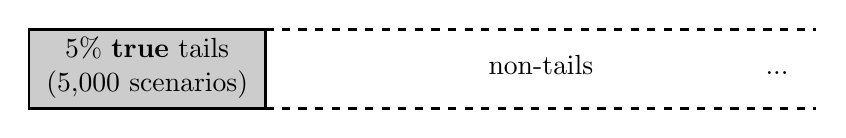
\begin{tikzpicture}[scale=1]
            % Make the height of the solid rectangle half.
            \draw[line width=1pt, fill=gray, fill opacity=0.40] (0,0) rectangle (3,1); 
            % Adjust node positions for the new height.
            \node[above] at (1.5, 0.5) {5\% \textbf{true} tails}; 
            \node[above] at (1.5, 0) {(5,000 scenarios)};
            % Adjust the dashed lines for the new height.
            \draw[dashed, line width=1pt] (3,0) -- (10,0); 
            \node[above] at (6.5, 0.3) {non-tails};
            \draw[dashed, line width=1pt] (3,1) -- (10,1); 
            \node[above] at (9.5, 0.3) {...};
        \end{tikzpicture}
    \end{figure}
    \begin{figure}
        \centering
        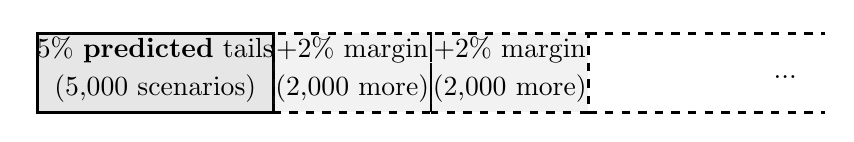
\begin{tikzpicture}[scale=1]
            % Make the height of the solid rectangle half.
            \draw[line width=1pt, fill=gray, fill opacity=0.20] (0,0) rectangle (3,1);
            % Adjust node positions for the new height.
            \node[above] at (1.5, 0.5) {5\% \textbf{predicted} tails};
            \node[above] at (1.5, 0) {(5,000 scenarios)};
            % Adjust the dashed boxes for the new height.
            \draw[dashed, line width=1pt, fill=gray, fill opacity=0.10] (3,0) rectangle (5,1);
            \node[above] at (4, 0.5) {+2\% margin};
            \node[above] at (4, 0) {(2,000 more)};
            \draw[dashed, line width=1pt, fill=gray, fill opacity=0.10] (5,0) rectangle (7,1);
            \node[above] at (6, 0.5) {+2\% margin};
            \node[above] at (6, 0) {(2,000 more)};
            % Adjust the dashed lines for the new height.
            \draw[dashed, line width=1pt] (7,0) -- (10,0);
            \draw[dashed, line width=1pt] (7,1) -- (10,1);
            \node[above] at (9.5, 0.3) {...};
        \end{tikzpicture}
        \caption{Illustration: a safety margin of $4\%$ ($m = 9000$)}
    \end{figure}
    
    Choosing a safety margin: a trade-off between accuracy and efficiency.
    \begin{itemize}
        \item   A lower margin: not enough tail identified.
        \item   A higher margin: more accurate CVaR estimate, but more budget needed to perform extensive inner simulations.
    \end{itemize}
    
\end{frame}

\begin{frame}{Tail Scenario Identification}

    \begin{figure}[H]
        \includegraphics[width=0.48\textwidth]{../project2/figures/tailMatches/regLN.png}
        \includegraphics[width=0.48\textwidth]{../project2/figures/tailMatches/nnLN.png}
        \caption{Tail scenario identification for regression and DNN metamodels}
    \end{figure}

    \begin{itemize}
        \item Traditional regression metamodels are \textbf{unable} to accurately identify tail scenarios even with high safety margins.
        \item LSTM metamodels surpasses the standard procedure with $5\%$ safety margin.
    \end{itemize}
        
\end{frame}

\begin{frame}{Estimating CVaR}
    
    \begin{figure}[H]
        \includegraphics[width=0.48\textwidth]{../project2/figures/CVaR/allLN.png}
        \includegraphics[width=0.48\textwidth]{../project2/figures/CVaR/zoomedLN.png}
        \caption{CVaR estimation for DNN metamodels}
    \end{figure}

    \begin{itemize}
        \item Traditional regression metamodels are \textbf{unable} to accurately estimate CVaR even with high safety margins.
        \item LSTM surpasses the standard procedure with a \textbf{5\% safety margin}.
        \item With a 95\% safety margin, any two-stage procedure produce the same CVaR estimate as a standard procedure.
    \end{itemize}

\end{frame}

\begin{frame}{Sensitivity Testing for DNNs}

    In a simulation study, we have control over the \textbf{noise level in training labels} and the \textbf{number of training samples}.

    \vspace{10pt}
    
    Controling the inner replications $N'$ varies the noise level in training labels.

    \begin{itemize}
        \item   \textbf{Low noise labels}: $N' = 100$
        \item   \textbf{Medium noise labels}: $N' = 10$
        \item   \textbf{High noise labels}: $N' = 1$
    \end{itemize}

    \vspace{10pt}

    Controling the outer scenarios $M$ varies the number of training samples.

    \begin{itemize}
        \item $M \in \{10^2, 10^3, 10^4, 10^5\}$
    \end{itemize}

    \vspace{10pt}

    2 LSTMs of \textbf{different capacities} are examined based on their MSEs.


\end{frame}

\begin{frame}{Noise Tolerance of DNNs}
    
    \begin{table}[ht!]
        \centering
        \begin{tabular}{lccccc}
            \toprule
            \textbf{Model}      & \textbf{$N'$}         & \textbf{Training error}                & \textbf{Test error}               & \textbf{True error}\\
            \midrule
            LSTM                & $100$                & $0.075$         & $0.079$     & $0.063$ \\ 
            High-capacity LSTM  & $100$                & $0.068$         & $0.102$     & $0.060$ \\
            Average Difference  & $100$                & $-0.007$       & $0.023$     & $-0.003$ \\
            \hline
            LSTM                & $10$                 & $0.195$         & $0.193$     & $0.070$ \\
            High-capacity LSTM  & $10$                 & $0.157$         & $0.199$     & $0.065$ \\
            Average Difference  & $10$                 & $-0.038$       & $0.006$     & $-0.005$ \\
            \hline
            LSTM                & $1$                  & $1.366$         & $0.781$     & $0.129$ \\
            High-capacity LSTM  & $1$                  & $1.354$         & $0.795$     & $0.149$ \\
            Average Difference  & $1$                  & $-0.012$       & $0.014$     &\textcolor{color10_5}{$0.020$} \\
            \bottomrule
        \end{tabular}
        \caption{MSEs of LSTM metamodels.}
    \end{table}

    \begin{itemize}
        \item   Both LSTMs cut through the noise in training labels.
        \item   Both LSTMs deteriorate dramatically on \textbf{high-noise} labels.
        \item   High-capacity LSTM can tolerate \textbf{low} and \textbf{medium} label noise.
    \end{itemize}

\end{frame}

\begin{frame}{Noise Tolerance of DNNs}

    \begin{figure}[ht!]
        \centering
        \includegraphics[width=\textwidth]{../project2/figures/qqPlots/lstmAll.png}
    \end{figure}

\end{frame}

\begin{frame}{Sensitivity of Regular LSTM}

    \begin{table}[ht!]
        \centering
        \begin{tabular}{lccccc}
            \toprule
                           & $N'=1$   & $N'=10$  & $N'=100$ & $N'=1000$\\
            \midrule
            $M = 100$      & \textcolor{color10_2}{$1.139$} & \textcolor{color10_3}{$0.229$} & \textcolor{color10_4}{$0.167$} & \textcolor{color10_5}{$0.158$} \\
            $M = 1000$     & \textcolor{color10_3}{$0.559$} & \textcolor{color10_4}{$0.173$} & \textcolor{color10_5}{$0.123$} & \textcolor{color10_6}{$0.127$} \\
            $M = 10000$    & \textcolor{color10_4}{$0.283$} & \textcolor{color10_5}{$0.115$} & \textcolor{color10_6}{$0.099$} & \textcolor{color10_7}{$0.097$} \\
            $M = 100000$   & \textcolor{color10_5}{$0.129$} & \textcolor{color10_6}{$0.070$} & \textcolor{color10_7}{$0.063$} & \textcolor{color10_8}{$0.063$} \\
            \bottomrule
        \end{tabular}
        \caption{MSE between regular LSTM's predicted losses and true losses.}
    \end{table}

    \begin{itemize}
        \item   Same color $\rightarrow$ same total simulation budget.
        \item   $N = 10$ is a reasonable budget allocation for LSTM metamodels.
    \end{itemize}
    
\end{frame}

\begin{frame}{Sensitivity of High-capacity LSTM}

    \begin{table}[ht!]
        \centering
        \begin{tabular}{lccccc}
            \toprule
            & $N'=1$ & $N'=10$  & $N'=100$ & $N'=1000$\\
            \midrule
            $M = 100$      & \textcolor{color10_2}{$0.764$} & \textcolor{color10_3}{$0.408$} & \textcolor{color10_4}{$0.131$} & \textcolor{color10_5}{$0.087$} \\
            $M = 1000$     & \textcolor{color10_3}{$0.878$} & \textcolor{color10_4}{$0.367$} & \textcolor{color10_5}{$0.156$} & \textcolor{color10_6}{$0.087$} \\
            $M = 10000$    & \textcolor{color10_4}{$0.351$} & \textcolor{color10_5}{$0.147$} & \textcolor{color10_6}{$0.064$} & \textcolor{color10_7}{$0.063$} \\
            $M = 100000$   & \textcolor{color10_5}{$0.149$} & \textcolor{color10_6}{$0.065$} & \textcolor{color10_7}{$0.060$} & \textcolor{color10_8}{$0.038$} \\
            \bottomrule
        \end{tabular}
        \caption{MSE between high-capacity LSTM's predicted losses and true losses.}
    \end{table}

    \begin{itemize}
        \item   Same color $\rightarrow$ same total simulation budget.
        \item   $N' = 10$ is a reasonable budget allocation for LSTM metamodels.
    \end{itemize}
    
\end{frame}

\begin{frame}{Single-Stage Procedure}

    \begin{figure}[ht!]
        \centering
        \includegraphics[width=0.48\textwidth]{../project2/figures/singleStage/CVaRmediumNoise.png}
        \includegraphics[width=0.48\textwidth]{../project2/figures/singleStage/CVaRhighNoise.png}
        \caption{CVaR estimates of single-stage procedures (left: $N' = 10$. right: $N' = 1$).}
    \end{figure}

    \begin{itemize}
        \item   The single-stage procedure outperforms the two-stage procedure.
        \item   The single-stage procedure is more efficient than the two-stage procedure.
        \item   Setting $N' = 10$ is a reasonable budget allocation.
    \end{itemize}

\end{frame}

\begin{frame}{Convergence Analysis}

    For each $\Gamma$, the best performing metamodel is used.

    \begin{itemize}
        \item   Maximum number of outer scenarios $M = 10^5$.
    \end{itemize}

    \begin{figure}[ht!]
        \centering
        \includegraphics[width=0.48\textwidth]{../project2/figures/singleStage/MSEConvergence_lstmLoCap.png}
        \includegraphics[width=0.48\textwidth]{../project2/figures/singleStage/MSEConvergence_lstmHiCap.png}
        \caption{Empirical convergence of CVaR for single-stage procedures with LSTM metamodels (left: regular LSTM. right: high-capacity LSTM).}
    \end{figure}

    \begin{itemize}
        \item   Minimal effect of increasing $N'$ on CVaR estimation.
        \item   Similar behavior as regression metamodels ($d=20$) in the previous section.
    \end{itemize}

\end{frame}

\begin{frame}{Convergence Analysis}
    \begin{figure}[ht!]
        \centering
        \includegraphics[width=\textwidth]{../project2/figures/singleStage/MSEConvergence_lstmLoCap_MN.png}
        \caption{Empirical convergence of the single-stage procedure with a LSTM metamodel.} 
    \end{figure}

    \begin{itemize}
        \item   Minimal effect of increasing $N'$ on CVaR estimation.
        \item   For a given $\Gamma$, set $N'$ constant and allocate budget to outer simulations.
    \end{itemize}

\end{frame}

\begin{frame}{Conclusion}

    \textbf{Key Findings:}
    \begin{itemize}
        \item   LSTMs are \textbf{resilient} to moderate levels of noise in training labels.
        \item   Deep neural networks can learn \textbf{true} complex dynamic hedging model.
        \item   Two-stage procedure addresses regulatory concerns by avoiding direct use of metamodel predictions.
        \item   Single-stage procedure is \textbf{efficient} and \textbf{versatile}.
        \item   \textbf{Increasing outer scenarios} is more beneficial.
        \item   High-capacity LSTM requires lower noise training labels.
    \end{itemize}

    \vspace{10pt}

    \textbf{Future Directions:}
    \begin{itemize}
        \item   Apply deep neural network metamodels to other risk management tasks.
        \item   Investigate impact of label noise on other deep learning models 
        \item   Explore optimal network architectures for different simulation models.
    \end{itemize}
    
\end{frame}


\section{Transfer Learning for Rapid Adaptation of DNN Metamodels}
\begin{frame}{Transfer Learning for Rapid Adaptation of DNN Metamodels}

    \textbf{Challenge:} Adapting deep neural network metamodels to changing conditions.
    \begin{itemize}
        \item   Retraining from scratch is computationally expensive.
        \item   Efficient incorporation of new VA contract data.
        \item   Balancing model accuracy and computational costs.
    \end{itemize}

    \vspace{10pt}

    \textbf{Solution:} Transfer learning (TL) to develop adaptable, efficient metamodels for VA dynamic hedging.

    \begin{itemize}
        \item   Pre-train deep neural network on contracts with abundant simulation data.
        \item   Fine-tune on smaller dataset of new contracts/market conditions.
        \item   Leverages shared features between VA contracts.
        \item   Computational savings:
            \begin{itemize}
                \item   Reduced training time.
                \item   Fewer data points needed for good performance.
            \end{itemize}
    \end{itemize}

\end{frame}


\begin{frame}{Transfer Learning Framework}

    \textbf{Key Components:}
    \begin{itemize}
        \item   \textbf{Domain} $\mathcal{D}$: feature space $\mathcal{X}$ + probability distribution $F$
        \item   \textbf{Task} $\mathcal{T}$: label space $\mathcal{Y}$ + predictive function $f: \mathcal{X} \rightarrow \mathcal{Y}$
    \end{itemize}

    \vspace{10pt}
    \textbf{Source vs. Target:}
    \begin{itemize}
        \item   \textbf{Source:} $\mathcal{D}_{\text{So}} = \{\mathcal{X}_{\text{So}}, F_{\text{So}}(X)\}$
        \item   \textbf{Target:} $\mathcal{D}_{\text{Ta}} = \{\mathcal{X}_{\text{Ta}}, F_{\text{Ta}}(X)\}$
    \end{itemize}

    \vspace{10pt}
    \textbf{Our Goal:}
    \begin{itemize}
        \item   \textbf{Input features} $X$: risk factors from outer simulation
        \item   \textbf{Output labels} $L$: contract losses
        \item   \textbf{Source and target}: from VAs with abundant simulation data to new VAs with limited data
        \item   \textbf{Goal}: improve $f_{\text{Ta}}(\cdot)$ using knowledge from $\mathcal{D}_{\text{So}}$ and $f_{\text{So}}(\cdot)$
    \end{itemize}

\end{frame}

\begin{frame}{Transfer Learning Techniques}

    \textbf{Common Techniques:}
    \begin{itemize}
        \item   \textbf{Fine-tuning:} a model pre-trained on a source task is used as a starting point for a target task.
        \item   \textbf{Layer freezing:} only part of the model is fine-tuned.
        \item   \textbf{Multi-task learning:} perform training on multiple tasks simultaneously.
    \end{itemize}

    \vspace{10pt}

    \textbf{Key considerations:}
    \begin{itemize}
        \item   Similarity between source and target tasks
        \item   Appropriate learning rate
    \end{itemize}

\end{frame}

\begin{frame}{Fine-tuning Algorithm for LSTM Metamodels in VA Hedging}

    \begin{algorithm}[H]
        \caption{Fine-tuning Algorithm for LSTM Metamodels in VA Hedging}
        \begin{algorithmic}[1]
            \STATE \textbf{Input:} $\mathcal{D}_{\text{So}} = \{(X_{\text{So}}^{(i)}, L_{\text{So}}^{(i)})\}_{i=1}^{M_{\text{So}}}$ , $\mathcal{D}_{\text{Ta}} = \{(X_{\text{Ta}}^{(i)}, L_{\text{Ta}}^{(i)})\}_{i=1}^{M_{\text{Ta}}}$, $\alpha_{\text{So}}$, and $\alpha_{\text{Ta}}$.
            \STATE Train a LSTM metamodel $f_{\text{So}}(\cdot; \theta_{\text{So}})$ on $\mathcal{D}_{\text{So}}$:
            \begin{equation*}
                \theta_{\text{So}} = \min_{\theta} \frac{1}{M_{\text{So}}} \sum_{i=1}^{M_{\text{So}}} \left( f_{\text{So}}(X_{\text{So}}^{(i)}; \theta) - L_{\text{So}}^{(i)} \right)^2
            \end{equation*}
            \STATE Initialize the target metamodel parameters $\theta_{\text{Ta}}$ using the pre-trained metamodel parameters:
            \begin{equation*}
                \theta_{\text{Ta}} \gets \theta_{\text{So}}
            \end{equation*}
            \STATE Fine-tune the entire LSTM metamodel $f_{\text{Ta}}(\cdot; \theta_{\text{Ta}})$ on the target dataset $\mathcal{D}_{\text{Ta}}$ using a smaller learning rate $\alpha_{\text{Ta}}$:
            \begin{equation*}
                \theta_{\text{Ta}} = \min_{\theta} \frac{1}{M_{\text{Ta}}} \sum_{i=1}^{M_{\text{Ta}}} \left( f_{\text{Ta}}(X_{\text{Ta}}^{(i)}; \theta) - L_{\text{Ta}}^{(i)} \right)^2
            \end{equation*}
            \STATE \textbf{Output:} Final adapted LSTM metamodel $f_{\text{Ta}}(\cdot; \theta_{\text{Ta}})$ for the target task
        \end{algorithmic}
    \end{algorithm}

\end{frame}

\begin{frame}{Layer Freezing Algorithm for LSTM Metamodels in VA Hedging}

    \begin{algorithm}[H]
        \caption{Layer Freezing Algorithm for LSTM Metamodels in VA Hedging}
        \begin{algorithmic}[1]
            \STATE \textbf{Input:} $\mathcal{D}_{\text{So}} = \{(X_{\text{So}}^{(i)}, L_{\text{So}}^{(i)})\}_{i=1}^{M_{\text{So}}}$ , $\mathcal{D}_{\text{Ta}} = \{(X_{\text{Ta}}^{(i)}, L_{\text{Ta}}^{(i)})\}_{i=1}^{M_{\text{Ta}}}$, $\alpha_{\text{So}}$, and $\alpha_{\text{Ta}}$.
            \STATE Train LSTM model $f_{\text{So}}(\cdot; \theta_{\text{So}})$ on $\mathcal{D}_{\text{So}}$.
            \STATE Initialize the target model parameters $\theta_{\text{Ta}} = [\theta_0, \theta_1]$ using the pre-trained source model parameters $\theta_{\text{So}}$:
            \begin{equation*}
                \theta_{\text{Ta}} \gets \theta_{\text{So}} = [\theta_0, \theta_1]
            \end{equation*}
            \STATE Freeze the parameters of the shared layers $\theta_0$ and fine-tune the trainable layers $\theta_1$ on the target dataset $\mathcal{D}_{\text{Ta}}$:
            \begin{equation*}
                \theta_{\text{Ta}} = \min_{\theta_1} \frac{1}{M_{\text{Ta}}} \sum_{i=1}^{M_{\text{Ta}}} \left( f_{\text{Ta}}(X_{\text{Ta}}^{(i)}; [\theta_0, \theta_1]) - L_{\text{Ta}}^{(i)} \right)^2
            \end{equation*}
            \STATE \textbf{Output:} Adapted model $f_{\text{Ta}}(\cdot; \theta_{\text{Ta}})$ for the target task.
        \end{algorithmic}
    \end{algorithm}

\end{frame}

\begin{frame}{Multi-task Learning Algorithm for LSTM Metamodels in VA Hedging}

    \begin{algorithm}[H]
        \caption{Multi-task Learning Algorithm for LSTM Metamodels in VA Hedging}
        \begin{algorithmic}[1] \label{alg3:multiTaskLearning}
            \STATE \textbf{Input:} learning rate $\alpha$, set of $K$ tasks $\{\mathcal{T}_k\}_{k=1}^K$ with datasets $\mathcal{D}_k = \{(X_k^{(i)}, L_k^{(i)})\}_{i=1}^{M_k}$, task-specific parameters $\theta_k$ for each task $k$, and shared parameters $\theta_0$.
        
            \STATE Train the multi-head LSTM metamodel on all $K$ tasks simultaneously by minimizing the multi-task loss function:
            \begin{equation} \label{eq3:multiTaskLoss}
                \min_{\theta_0, \{\theta_k\}_{k=1}^K} \sum_{k=1}^K \frac{1}{M_k} \sum_{i=1}^{M_k} \left( f_i(X_k^{(i)}; \theta_0, \theta_k) - L_k^{(i)} \right)^2
            \end{equation}
        
            \STATE Update both the shared parameters $\theta_0$ and task-specific parameters $\{\theta_k\}_{k=1}^K$ simultaneously using backpropagation and gradient descent with learning rate $\alpha$.
            
            \STATE \textbf{Output:} Trained multi-task metamodel $f(\cdot; \theta_0, \{\theta_k\}_{k=1}^K)$ for all $K$ tasks
        \end{algorithmic}
    \end{algorithm}

\end{frame}

\begin{frame}{Experiment Setup}

    \begin{table}[ht!] 
        \centering
        \begin{tabular}{lcccc} 
        \toprule
        \textbf{Contract} & \textbf{Asset Model} & \textbf{Lapse} & \textbf{$M_{\text{So}}$}  & \textbf{$M_{\text{Ta}}$}\\
        \midrule
        GMMB & GBM & No lapse & 50000 & N/A \\
        GMMB & RS-GBM & No lapse & 50000 & 2000 \\
        GMMB & RS-GBM & Static lapse & 50000 & 2000 \\
        GMMB & RS-GBM & Dynamic lapse & 50000 & 2000 \\
        GMWB & RS-GBM & Dynamic lapse & N/A & 2000 \\
        \bottomrule
        \end{tabular}
        \caption{VA Contracts for Transfer Learning Experiments}
    \end{table}

    We aim to examine the performance of TL techniques
    \begin{itemize}
        \item   learning the lapse features,
        \item   learning the dynamic lapse, and 
        \item   transferring to other contract types.
    \end{itemize}

\end{frame}



\begin{frame}{Learning Lapse Features}
    \begin{figure}[ht!]
        \centering
        \begin{subfigure}{0.48\textwidth}
            \includegraphics[width=\textwidth]{../project3/figures/figure1a.png}
            \caption{Extensive Training on Target Task}
        \end{subfigure}
        \begin{subfigure}{0.48\textwidth}
            \includegraphics[width=\textwidth]{../project3/figures/figure1b.png}
            \caption{Without TL}
        \end{subfigure}
        \caption{Direct training on RS-GBM GMMB with static lapse}
    \end{figure}
\end{frame}

\begin{frame}{Learning Lapse Features}
    \begin{figure}[ht!]
        \centering
        \begin{subfigure}{0.48\textwidth}
            \includegraphics[width=\textwidth]{../project3/figures/figure1c.png}
            \caption{With Fine-tuning}
        \end{subfigure}
        \begin{subfigure}{0.48\textwidth}
            \includegraphics[width=\textwidth]{../project3/figures/figure1d.png}
            \caption{With Layer Freezing}
        \end{subfigure}
        \caption{TL on RS-GBM GMMB with static lapse}
    \end{figure}

\end{frame}



\begin{frame}
    \frametitle{References}
    \bibliographystyle{apa}
    \bibliography{../refP1, ../refP2, ../refP3}
\end{frame}
\end{document}